Each Arabic letter represents a consonant, which means that short vowels are not
represented by the 36 characters, for this reason, the need of \textit{diacritics}
rises. \textit{Diacritics} are symbols that comes after a letter to state the
short vowel accompanied by that letter. There are four diacritics \textarabic{◌َ} \textarabic{◌ُ}
\textarabic{◌ِ} \textarabic{◌ْ} which represent the following short vowels
/\textit{a}/, /\textit{u}/, /\textit{i}/ and \textit{no-vowel} respectively,
their names are \textit{fat-ha, dam-ma, kas-ra and sukun} respectively.  The first
three symbols are called \textit{harakat}. Table~\ref{tables:diacritics_dal}
shows the 4 diacritics on a letter.



% table: dal with diacritics
\begin{table}[!t]
	\centering
	\begin{tabular}{c c c c c c}
		%\hline
		\toprule
		\textbf{\small{Diacritics}}     & \small{\textit{without}} & \small{\textit{fat-ha}} &
		\small{\textit{kas-ra}} & \small{\textit{dam-ma}} & \small{\textit{sukun}}\\
		%\hline
		\midrule
		\textbf{\small{Shape}}   & \textarabic{د} & \textarabic{دَ} & \textarabic{دِ} &
		\textarabic{دُ} & \textarabic{دْ}\\
		%\hline
		\bottomrule
	\end{tabular}
	\caption{Diacritics on the letter  \textarabic{ د }}\label{tables:diacritics_dal}
\end{table}



There are two more sub-diacritics made up of the basic four to represent two
cases:
\begin{definition}\label{def:shadaa_definition}
  \textbf{Shadaa}  \hfill \\
to indicate the letter is doubled. Any letter with
shaddah (\textarabic{ ّ } ) the letter should be duplicated: first letter with a
constant (sukoon) and second letter with a vowel (haraka)~\cite{Alnagdawi2013}; Table ~\ref{tables:shadda_dal}
shows the dal with shadda and the original letters.
% table: dal with shadda

\begin{table}[!t]
	\centering
	\begin{tabular}{c c c}
		%\hline
		\toprule
		\textbf{\small{Diacritics}} & \small{\textit{letter with Shadda }} & \small{\textit{letters without shadaa  }} \\
		%\hline
		\midrule
		\textbf{\small{Shape}}  & \textarabic{دَّ} &  \textarabic{دْدَ}\\
		%\hline
		\bottomrule
	\end{tabular}
	\caption{Shadaa diacritics on the letter  \textarabic{ د }}\label{tables:shadda_dal}
\end{table}

\end{definition}

\begin{definition}\label{def:tanween_definition}
  \textbf{Tanween} \hfill \\
  %%%~\ref{defa} and~\ref{defb}
  is doubling the short vowel, and can convert
Tanween fathah, Tanween dhammah or Tanween kasrah by
replacing it with the appropriate vowel ( ُ◌ – dhammah, َ◌ –
fathah or ِ◌ –kasrah ) then add the Noon letter with constant to the end of the word~\cite{Alnagdawi2013}. Table~\ref{tables:Tanween_dal}
shows the difference between the original letter and the letter with Tanween

\begin{table}[!t]
	\centering
	\begin{tabular}{c c c}
		%\hline
		\toprule
		\textbf{\small{Diacritics}} & \small{\textit{letter with tanween }} & \small{\textit{letters without tanween}} \\
		%\hline
		\midrule

          \textbf{\small{Tanween Fat-ha}}  & \textarabic{دً} &  \textarabic{دَ+نْ}\\
          \textbf{\small{Tanween Dam-ma}}  & \textarabic{دٌ} &  \textarabic{دُ+نْ}\\
          \textbf{\small{Tanween Kas-ra}}  & \textarabic{دٍ} &  \textarabic{دِ+نْ}\\


		\bottomrule
	\end{tabular}
	\caption{Tanween diacritics on the letter  \textarabic{ د }} \label{tables:Tanween_dal}
\end{table}


\end{definition}

 Arabs pronounce the sound \textit{/n/} accompanied \textit{sukun} at the end the indefinite words, that sound corresponds to this
letter \textarabic{نْ}, it is called \textit{noon-sakinah}, however, it is
just a phone, it is not a part of the indefinite word, if a word comes as a
definite word, no additional sound is added. Since it is not an essential sound,
it is not written as a letter, but it is written as  \textit{tanween}
\textarabic{◌ٌ ◌ً ◌ٍ}.
% adding tanween and its relationship to the previous letter
\textit{Tanween} states the sound \textit{noon-sakinah}, but as you have noticed,
there are 3 \textit{tanween} symbols, this because  \textit{tanween} is added as
a diacritic over the last letter of the indefinite word, one of the 3 harakat\textit{harakat} accompanies the last letter, the last letter's \textit{harakah}
needs to be stated in addition to the sound \textit{noon-sakinah}, so
\textit{tanween} is doubling the last letter's \textit{haraka}, this way the last
letter's \textit{haraka} is preserved in addition to stating the sound
\textit{noon-sakinah}; for example, \textarabic{رَجُلُ + نْ} is written
\textarabic{رَجُلٌ} and  \textarabic{رَجُلِ + نْ} is written \textarabic{رَجُلٍ}.


Those two definition, Definition ~\ref{def:shadaa_definition} and Definition ~\ref{def:tanween_definition}  will help us to reduce the dimension of the letter's feature vector as we will see in \textit{preparing data} section.


Diacritics makes short vowels clearer, but they are not necessary.
Moreover, a phrase without full diacritics or with just some on some letters is
right linguistically, so it is allowed to drop them from the text.

% Diacritics in Unicode
In Unicode, Arabic diacritics are standalone symbols, each of them has its own
unicode. This is in contrast to the Latin diacritics; e.g., in the set
\textit{\{ê, é, è, ë, ē, ĕ, ě\}}, each combination of the letter \textit{e} and a diacritic is represented by one unicode.



\section{Arabic Arud}
% @@@ add el3elal and zahafat
% @@@ add tent picture
% @@@ add details into every bahr
 


\begin{definition}\label{def:arud}
  \textbf{Arud} \hfill \\
  In Arabic Arud natively has many meanings (the way, the direction, the light clouds and Mecca and Madinah \footnote{\textit{Mecca and Madinah are two cities in  Saudi Arabia}.}~\cite{AlQuaed}. Arud is the study of Arabic Poem meters and the rules which confirm if the Poem is sound meters \& broken meters.
\end{definition}
 
The Author of Arabic Arud  is \textit{Al-Farahidi} (718 – 786 CE) who analyzed the Arabic poetry; then he came up with that the succession of consonants and vowels produce patterns or \textit{meters}, which make the music of poetry. He was one of the famous people who know The melodies and the musical parts of speech. He ha counted them fifteen meters.  After that, a student of \textit{Al-Farahidi} has added one more meter to make them sixteen. Arabs call meters \textarabic{بحور} which means "\textit{seas}" Poets have written poems without knowing exactly what rules which make a collection of words a poem.

The Reasons which makes \textit{Al-Farahidi} put this rules is

  \begin{itemize}
  \item Protect the Arabic Poetry from the broken meters.
  \item Distinguish between the original Arabic Poetry and the not original Arabic Poetry or from the prose.
    \item Make the rules clear and easy for anyone who needs to write a poem.
  \end{itemize}

  Some people said that the one-day Al-Farahidi was walking into the metal-market and he was said some of the poetry and for some reasons the knock of the metals matched the musical sound of the poetry he was saying then he got an idea to explore the Arud of the poetry.

 There are many reason for Arud name 
  \begin{itemize}
  \item It named Arud because some people said he put this rules in Arud place \textarabic{العَروض} \textit{with fat-ha, not with dam-ma such as the rules name \textarabic{العُروض} } between Mecca and Al-Ta'if\cite{AlQuaed}.
  \item Arud in Arabic is noun come from verb \textarabic{يعرض} which means here to be assessed. They said because of Any poem should be assessed by Al-Arud rules so, it named Al-Arud~\cite{Alkafi1994}.
  \end{itemize}
  
  

  
    
    \subsection{Al-Farahidi and Pattern Recognition}
    This subsection is our opinion in Al-Farahidi and his method he followed during working on Arabic Poetry Meter Classification.

\begin{enumerate}


\item Al-Farahidi thought there is a pattern for every collection of the poetry by chance; however, He rigorously worked into this problem. He started analyzing the poetry and add every group with the same tafa'il to the same class.
\item He analyzed the outliers and the particular case from every class and added it to his model.
\item He revised the meters and get the cases and generalize his case to be fit into all poetry.
\item His student once he found some poetry which was not fit into any model to be a model for a new class.

\end{enumerate}
The best essential point which made us admired by Al-Farahidi is his way of research and his passion for getting an indeed succession model. Also, his model is general and followed all the steps currently any Data scientist follows to explore new pattern. Some people state that He died when he was thinking about the problem he hit a wall which made trouble for him. His die story shows that he was thinking in profoundly about this problem. One of the most interest thing I found during this research is how he found this pattern and Al-Farahidi’s way to find a new thing.
%@@@ add about student for sebayeah
%@@@ التأكد من أن القرآن والحديث ليس شعر وﻹن تصادف فهو ليس قصداً والشعر يجب أن يكون وزناً إتفاقاً

    
    
    \subsection{Feet Representation}
    A meter is an ordered sequence of feet. Feet are the basic
units of meters; there are ten of them.
\begin{definition}\label{def:feet}
  \textbf{Feet} \hfill \\  A Foot consists of
a sequence of \textbf{Sukun} (Consonants) represented as (0) and \textbf{Harakah} (Vowels) (/). Traditionally, feet are represented by mnemonic words called tafa’il \textarabic{تفاعيل}.
\end{definition}

feet consists of three parts (Asbab (means Reasons in English) \textarabic{أسباب}, Awtaad (means Wedges in English) \textarabic{وتد}, Fawasel (means Breaks in English) \textarabic{فواصل}).
\begin{itemize}
\item \textbf{Reasons (\textarabic{أسباب})}: It has two types
  \begin{enumerate}
  \item \textbf{Light (\textarabic{سبب خفيف})} which happens when we have the first letter is harakah and the second is sukun (/0) example (\textarabic{هَبْ, لَمْ}).
    \item \textbf{Heavy (\textarabic{سبب ثقيل})} which happens when we have two harakah letter (//) example (\textarabic{لَكَ, بِكَ}).
    \end{enumerate}
    \item \textbf{Wedge (\textarabic{وتد})}: It has two types
  \begin{enumerate}
  \item \textbf{Combined Wedge (\textarabic{وتد مجموع})} which happens when we have two harakah letters followed by sukun (//0) example (\textarabic{مَشَى, عَلَى}).
    \item \textbf{Separated Wedge (\textarabic{وتد مفروق})} which happens when we have two harakah and in between a sukun letter (/0/) example (\textarabic{مُنْذُ, مِصْرُ}).
    \end{enumerate}
    \item \textbf{Breaks (\textarabic{فواصل}}): It has two types
  \begin{enumerate}
  \item \textbf{Small Break (\textarabic{فاصلة صغرى}}) which happens when we have three harakah letters followed by a sukun letter (///0) example (\textarabic{ذَهَبُوا, سُفُناً}).
    \item \textbf{Big Break (\textarabic{فاصلة كبرى}}) which happens when we have four harakah letters followed by a sukun letter  (////0) example (\textarabic{جَعَلَهُمْ}).\footnote{\textit{Some of Arab linguistic scientist assume the small Breaks as a combination between big reason and small reason. Same for the Big Breaks assumed to be a combination between Big reason and Combined Wedge. So, they didn't assume we have three types of feet it is only pure two and any other feet constructed from this two. In this thesis we assume there are three feet }.}
    \end{enumerate}
  \end{itemize}


  \subsubsection{Rules for Arabic Letters Representation}
  Arabic Arud has one general rule in the poetry representation which is we represent only the letters which is (spoken) not the written which means the letters with phonatics not the written. We have give the below rules as a results of the general rule.

  \begin{itemize}
  \item Any letter with \textit{harakah} represented as (/).
  \item Any letter with \textit{sukun} represented as (0).
  \item Any letter with shaddah represented by two letters the first one will be \textit{sukun} and the second letter will be \textit{harakah} represented as (0/) example (\textarabic{مُحَمََّد}) will be (//0//0).
  \item Any letter with tanween represented by two letters the first one is \textit{haraka} (/) and the second is \textit{sukun}.
  \item Alef without hamze (\textarabic{همزة الوصل}) and Wow Algmaa are not represented example (\textarabic{وُاعلَموا}) will be (/0//0)
  \item If we have a letter which is not written but (spoken) so, we will represent it example (\textarabic{هذا}) it include Alef but not written (\textarabic{هاذا}) the representation will be (/0/0).
  \item If we have \textit{Meem Aljamaa} with harakah so, it represented with \textit{Mad} example (\textarabic{هُمُ}) will be (//0) .
  \item \textit{Alef Mad} (\textarabic{آ}) will be two letters \textit{Alef with harakah} and \textit{Alef with sukun} example (\textarabic{آدَمُ}) will be (/0//).
    \item if the verse ended with \textit{harkah} we will add \textit{sukun} to it.


    \end{itemize}
Example: (note: the below representation first line is simliar the second one but with Arud language style ).
\begin{Arabic}
  \begin{traditionalpoem*}
أرَاكَ عَصِيَّ الدّمعِ شِيمَتُكَ الصّبرُ،\quad & \quad أما للهوى نهيٌ عليكَ ولا أمرُ ؟
أرَاكَ عَصيْيَ دّمعِ شِيمَتُكَ صّبرُو،\quad & \quad أما للهوى نهينْ عليكَ ولا أمرو ؟
	\end{traditionalpoem*}
\end{Arabic}
%@@@ add example the difference between arud writting and the actual writing


\subsection{Arabic Poetry feet}

Arabic poetry feet has ten tafa'il \textarabic{تفاعيل} (scansion)  any peom constructed from these feet. They are eight from writing (syntax) perspective, But it ten in the rules.
\begin{savenotes}

\begin{table}[!t]
  \centering
  \begin{tabular}{c c c c}
    \hline
    \textbf{\#} & \textbf{Feet} & \textbf{Scansion} & \textbf{Construction} \\
    \hline
    1 & \textarabic{فَعُولُنْ}  & \texttt{0/0//} & combined wedge (\textarabic{فعو}) and small reason (\textarabic{لن})   \\
    2 &\textarabic{مَفاعِيلُنْ}& \texttt{0/0/0//} & combined wedge (\textarabic{مفا}) and two light reasons (\textarabic{عي}) (\textarabic{لن})   \\
    3 &\textarabic{مُفَاعَلَتُنْ}& \texttt{0///0//}  &    combined wedge (\textarabic{مفا}), heavy reason (\textarabic{عل}) and light reason (\textarabic{تن}) \\
    4 &\textarabic{فَاعِلاَتُنْ} & \texttt{0/0//0/}   & light reason (\textarabic{فا}), combined wedge (\textarabic{علا}) and light reason (\textarabic{تن})   \\
    5 &\textarabic{فَاعِ لاتُنْ} & \texttt{0/0//0/}  &  Separated wedge (\textarabic{فاع}) and two light reason (\textarabic{لا})(\textarabic{تن}) \footnote{\textit{We separated the letters (\textarabic{ع}) and (\textarabic{لا}) in (\textarabic{فاع لاتن}) to show that this part is separated wedge and distinguish between this feet  and (\textarabic{فاع لاتن}) which contains combined wedge  }.}  \\
    6 &\textarabic{فَاعِلُنْ}  & \texttt{0//0/}   & light reason (\textarabic{فا}) and combined wedge (\textarabic{علن})\\
    7 &\textarabic{مُتَفَاعِلُنْ}& \texttt{0//0///}  & heavy reason (\textarabic{مت}), light reason (\textarabic{فا}) and combined wedge (\textarabic{علن})  \\
    8 &\textarabic{مَفْعُولاَت} & \texttt{0//0///}   & two light reason (\textarabic{مف})(\textarabic{عو}) and separated wedge (\textarabic{لات}) \\
    9 &\textarabic{مُسْتَفْعِلُنْ} & \texttt{0//0/0/}  &  two light reason (\textarabic{مس})(\textarabic{تف}) and combination wedge (\textarabic{علن}) \\
    10 &\textarabic{مُسْتَفْعِ لُنْ} & \texttt{0//0/0/}  & light reason (\textarabic{مس}), separated wedge  (\textarabic{تفع}) and light reason  (\textarabic{لن})\footnote{\textit{We separated the letters (\textarabic{ع}) and (\textarabic{ل}) in (\textarabic{مستفع لن}) to show that it ends with a separated wedge and distinguish between this feet  and (\textarabic{مستفعلن}) which contains combined wedge }}\\


    \hline
  \end{tabular}
  \caption{The ten feet of the Arabic meters. }\label{arud:feet}
\end{table}
    \end{savenotes}

%% Every digit (\texttt{/} or \texttt{0}) represents
%%    the corresponding diacritic over a letter in the feet. \texttt{/} corresponds to
%%    a\textit{harakah} ( \textarabic{◌َ}, \textarabic{◌ُ}, or \textarabic{◌ِ}) and \texttt{0}
%%    corresponds to a \textit{sukun} (\textarabic{◌ْ}). Any \textit{mad} (\textarabic{و, ا, ى}) is
%%    equivalent to \texttt{0}, \textit{tanween} is equivalent to \texttt{0/}, and \textit{shaddah} is
%%    equivalent to \texttt{/0}%

    
\begin{definition}\label{def:meter}
  \textbf{Meter} \hfill \\
  %%%% What is rtythm,feet
  Poetic meters define the basic rhythm of the poem. Each meter is described by a set of ordered feet which can be represented as ordered sets of consonants and vowels~\cite{Almuhareb2015}. A meter in Arabic named \textit{Bahr}   (\textarabic{بحر})
\begin{Arabic}
	\begin{traditionalpoem*}
          ولد الهدى فالكائنات ضياء\quad & \quad وفم الزمان تبسم وثناء انشاء
          الروح والملأ الملائك حوله\quad & \quad للدين والدنيا به بشراء

	\end{traditionalpoem*}
\end{Arabic}%
\end{definition}

\begin{definition}\label{def:verse}
  \textbf{Arabic Verse} \hfill \\ refers to "poetry" as contrasted to prose. Where the common unit of a verse is based on meter or rhyme, the common unit of prose is purely grammatical, such as a sentence or paragraph~\cite{Wiki_Verse}. A verse in Arabic named \textit{Bayt}(\textarabic{بيت})
\end{definition}

\begin{definition}\label{def:shatr}
  \textbf{Shatr} \hfill \\  A verse consists of two halves, each of them is called \textit{shatr} and carries the full meter.  We will use the term \textit{shatr} to refer to a verse's half; whether the right or the left half.
\end{definition}

\begin{definition}\label{def:poem}
  \textbf{Poem} \hfill \\  is a set of verses has the same meter and rhyme.
\end{definition}


\subsection{Arabic Poetry Meters}
\subsubsection{Al-Taweel \textarabic{الطويل}}
\textbf{tafa'il}
\begin{Arabic}
	\begin{traditionalpoem*}
          فعلون مفاعيلن فعولن مفاعلن\quad & \quad فعولن مفاعيلن فعولن مفاعيلن
	\end{traditionalpoem*}
      \end{Arabic}
      \textbf{Example:}

\begin{Arabic}
\begin{traditionalpoem}
أَمَاوِيَّ إِنَّ المَالَ غَادٍ وَرَائِحٌ\quad & \quad وَيَبْقَى مِنَ المَالِ الأحَادِيْثُ وَالذّكْرُ\\
{\color{purple} أَمَاوِيْ} {\color{blue} يَ إِنْنَ لْمَا} {\color{OliveGreen} لَ غَادِنْ} {\color{Brown} وَرَائِحُنْ}\quad & \quad
{\color{purple} وَيَبْقَى} {\color{blue} مِنَ لْمَالِ لـْ} {\color{OliveGreen} أَحَادِيـْ} {\color{Brown} ـثُ وَذْذِكْرُوْ}\\
{\color{purple} \texttt{//0/0}} {\color{blue} \texttt{//0/0/0}} {\color{OliveGreen} \texttt{//0/0}} {\color{Brown} \texttt{//0//0}}\quad & \quad
{\color{purple} \texttt{//0/0}} {\color{blue} \texttt{//0/0/0}} {\color{OliveGreen} \texttt{//0/0}} {\color{Brown} \texttt{//0/0/0}}\\
{\color{purple} فَعُوْلُنْ} {\color{blue} مَفَاعِيْلُنْ} {\color{OliveGreen} فَعُوْلُنْ} {\color{Brown} مَفَاعِلُنْ}\quad & \quad
{\color{purple} فَعُوْلُنْ} {\color{blue} مَفَاعِيْلُنْ} {\color{OliveGreen} فَعُوْلُنْ} {\color{Brown} مَفَاعِيْلُنْ}

\end{traditionalpoem}
\end{Arabic}

% % % % % % % % % % % % % % % % % % % % % % % % % % % % % % % % % % % % % % % % % % % % % % %

\subsubsection{Al-Madeed \textarabic{المديد}}
\textbf{tafa'il}

\begin{Arabic}
	\begin{traditionalpoem*}
فاعلاتن فاعلِن فاعلاتن\quad & \quad فاعلاتن فاعلن فاعلاتن
	\end{traditionalpoem*}
      \end{Arabic}
\textbf{Example:}
\begin{Arabic}
\begin{traditionalpoem}
مَنْ يُحِبَّ الْعِزَّ يَدْأّبْ إلَيْهِ\quad & \quad وَكَذَا مَنْ طَلَبَ الدُّرَّ غَاصَا\\
{\color{purple} مَنْ يُحِبْبَ لـْ} {\color{blue} ـعِزْزَ يَدْ} {\color{OliveGreen} أّبْ إلَيْهِيْ}\quad & \quad
{\color{purple} وَكَذَا مَنْ} {\color{blue} طَلَبَ دْ} {\color{OliveGreen} دُرْرَغَاصَا}\\
{\color{purple} \texttt{/0//0/0}} {\color{blue} \texttt{/0//0}} {\color{OliveGreen} \texttt{/0//0/0}}\quad & \quad
{\color{purple} \texttt{///0/0}} {\color{blue} \texttt{///0}} {\color{OliveGreen} \texttt{/0//0/0}}\\
{\color{purple} فَاْعِلاتُنْ} {\color{blue} فَاْعِلُنْ} {\color{OliveGreen} فَاْعِلاتُنْ}\quad & \quad
{\color{purple} فَعِلاتُنْ} {\color{blue} فَعِلُنْ} {\color{OliveGreen} فَاْعِلاتُنْ}
\end{traditionalpoem}
\end{Arabic}
% % % % % % % % % % % % % % % % % % % % % % % % % % % % % % % % % % % % % % % % % % % % % % %

\subsubsection{Al-Baseet \textarabic{البسيط}}
\textbf{tafa'il}
\begin{Arabic}
\begin{traditionalpoem*}
مستفعلن فعلن مستفعلن فاعلن\quad & \quad مستفعلن فاعلن مستفعلن فاعلن
\end{traditionalpoem*}
\end{Arabic}
\textbf{Example:}
\begin{Arabic}
\begin{traditionalpoem}
لايُعْجِبَنَّ مُضِيمًا حُسْنُ بِزّتهِ\quad & \quad وَهَلْ يَرُوقُ دَفينًا جَوْدَةُ الْكَفّنِ\\
{\color{purple} لايُعْجِبَنـْ} {\color{blue} نَ مُضِيـ} {\color{OliveGreen} ـمَنْ حُسْنُ بِزْ بِزْ} {\color{Brown} زَتِهِيْ}\quad & \quad
{\color{purple} وَهَلْ يَرُو} {\color{blue} قُ دَفِيْـ} {\color{OliveGreen} نَنْ جَوْدَةُ لـْ الـ} {\color{Brown} كَفَنِيْ}\\
{\color{purple} \texttt{/0/0//0}} {\color{blue} \texttt{///0}} {\color{OliveGreen} \texttt{/0/0//0}} {\color{Brown} \texttt{///0}}\quad & \quad
{\color{purple} \texttt{//0//0}} {\color{blue} \texttt{///0}} {\color{OliveGreen} \texttt{/0/0//0}} {\color{Brown} \texttt{///0}}\\
{\color{purple} مُسْتَفْعِلُنْ} {\color{blue} فَعِلُنْ} {\color{OliveGreen} مُسْتَفْعِلُنْ} {\color{Brown} فَعِلُنْ}\quad & \quad
{\color{purple} مُتفعلن} {\color{blue} فَعِلُنْ} {\color{OliveGreen} مُسْتَفْعِلُنْ} {\color{Brown} فَعِلُنْ}
\end{traditionalpoem}
\end{Arabic}

% % % % % % % % % % % % % % % % % % % % % % % % % % % % % % % % % % % % % % % % % % % % % % %
\subsubsection{Al-Wafer \textarabic{الوافر}}
\textbf{tafa'il}
\begin{Arabic}
\begin{traditionalpoem*}
مفاعلتن مفاعلتن مفاعلتن\quad & \quad مفاعلتن مفاعلتن مفاعلتن
\end{traditionalpoem*}
\end{Arabic}
\textbf{Example:}
\begin{Arabic}
\begin{traditionalpoem}
إِذَا لَمْ تَخْشَ عَاقِبَةَ اللَّيالِي\quad & \quad وَلَمْ تَسْتَحْيِ فَاصْنَعْ مَا تَشَاءُ\\
{\color{purple} إِذَا لَمْ تَخْـ} {\color{blue} ـشَ عَاقِبَةَ لـْ} {\color{OliveGreen} ـلَيالِيْ}\quad & \quad
{\color{purple} وَلَمْ تَسْتَحـْ} {\color{blue} ـيِ فَصْنَعْ مَا} {\color{OliveGreen} تَشَاءُوْ}\\
{\color{purple} \texttt{//0/0/0}} {\color{blue} \texttt{//0/0/0}} {\color{OliveGreen} \texttt{//0/0}}\quad & \quad
{\color{purple} \texttt{//0/0/0}} {\color{blue} \texttt{//0/0/0}} {\color{OliveGreen} \texttt{//0/0}}\\
{\color{purple} مُفَاْعَلْتُنْ} {\color{blue} مُفَاْعَلَتُنْ} {\color{OliveGreen} مُفَاْعَلْ}\quad & \quad
{\color{purple} مُفَاْعَلْتُنْ} {\color{blue} مُفَاْعَلَتُنْ} {\color{OliveGreen} مُفَاْعَلْ}
\end{traditionalpoem}
\end{Arabic}

% % % % % % % % % % % % % % % % % % % % % % % % % % % % % % % % % % % % % % % % % % % % % % %

\subsubsection{Al-Kamel \textarabic{الكامل}}
\textbf{tafa'il}

\begin{Arabic}
	\begin{traditionalpoem*}
متفاعلن متفاعلن متفاعلن\quad & \quad متفاعلن متفاعلن متفاعلن
	\end{traditionalpoem*}
      \end{Arabic}
\textbf{Example:}
\begin{Arabic}
\begin{traditionalpoem}
وَإِذَا صَحَوْتُ فَمَا أُقَصِّرُ عَنْ نَدًى\quad & \quad وَكَما عَلِمْتِ شَمَائِلِيْ وَتَكَرُّمِيْ\\
{\color{purple} وَإِذَا صَحَوْ} {\color{blue} تُ فَمَا أُقَصـْ} {\color{OliveGreen} ـصِرُ عَنْ نَدَنْ}\quad & \quad
{\color{purple} وَكَما عَلِمـْ} {\color{blue} ـتِ شَمَائِلِيْ} {\color{OliveGreen} وَتَكَرْرُمِيْ}\\
{\color{purple} \texttt{///0//0}} {\color{blue} \texttt{///0//0}} {\color{OliveGreen} \texttt{///0//0}}\quad & \quad
{\color{purple} \texttt{///0//0}} {\color{blue} \texttt{///0//0}} {\color{OliveGreen} \texttt{///0//0}}\\
{\color{purple} مُتَفَاْعِلُنْ} {\color{blue} مُتَفَاْعِلُنْ} {\color{OliveGreen} مُتَفَاْعِلُنْ}\quad & \quad
{\color{purple} مُتَفَاْعِلُنْ} {\color{blue} مُتَفَاْعِلُنْ} {\color{OliveGreen} مُتَفَاْعِلُنْ}
\end{traditionalpoem}
\end{Arabic}
% % % % % % % % % % % % % % % % % % % % % % % % % % % % % % % % % % % % % % % % % % % % % % %
\subsubsection{Al-Hazaj \textarabic{الهزج}}
\textbf{tafa'il}
\begin{Arabic}
\begin{traditionalpoem*}
مفاعيلن مفاعيلن\quad & \quad مفاعيلن مفاعيلن
\end{traditionalpoem*}
\end{Arabic}
\textbf{Example:}
\begin{Arabic}
\begin{traditionalpoem}
فَهُبُّوْا يَا بَنِيْ أُمِّيْ\quad & \quad إِلَى الْعَلْيَاءِ بالْعِلْمِ\\
{\color{purple} فَهُبْبُوْ يَا} {\color{blue} بَنِيْ أُمْمِيْ}\quad & \quad
{\color{purple} إلَ لْعَلْيَا} {\color{blue} ءِ بلْعِلْمِيْ}
{\color{purple} \texttt{//0/0/0}} {\color{blue} \texttt{//0/0/0}}\quad & \quad
{\color{purple} \texttt{//0/0/0}} {\color{blue} \texttt{//0/0/0}}\\
{\color{purple} مَفَاْعِيْلُنْ} {\color{blue} مَفَاْعِيْلُنْ}\quad & \quad
{\color{purple} مَفَاْعِيْلُنْ} {\color{blue} مَفَاْعِيْلُنْ}
\end{traditionalpoem}
\end{Arabic}
% % % % % % % % % % % % % % % % % % % % % % % % % % % % % % % % % % % % % % % % % % % % % % %
\subsubsection{Al-Rejz \textarabic{الرجز}}
\textbf{tafa'il}
\begin{Arabic}
\begin{traditionalpoem*}
مستفعلن مستفعلن مستفعلن\quad & \quad مستفعلن مستفعلن مستفعل
\end{traditionalpoem*}
\end{Arabic}
\textbf{Example:}
\begin{Arabic}
\begin{traditionalpoem}
لاخَيْرَ فِيْمَنْ كَفَّ عَنَّا شَرَّهُ\quad & \quad إِنْ كَانَ لايُرْجَى لِيَوْمٍ خَيْرُهُ\\
{\color{purple} لاخَيْرَ فِيْ} {\color{blue} مَنْ كَفْفَ عَنـْ} {\color{OliveGreen} ـنا شَرْرَهُوْ}\quad & \quad
{\color{purple} إِنْ كَانَ لا} {\color{blue} يُرْجَى لِيَوْ} {\color{OliveGreen} مِنْ خَيْرُهوْ}\\
{\color{purple} \texttt{/0/0//0}} {\color{blue} \texttt{/0/0//0}} {\color{OliveGreen} \texttt{/0/0//0}}\quad & \quad
{\color{purple} \texttt{/0/0//0}} {\color{blue} \texttt{/0/0//0}} {\color{OliveGreen} \texttt{/0/0//0}}\\
{\color{purple} مُسْتَفْعِلُنْ} {\color{blue} مُسْتَفْعِلُنْ} {\color{OliveGreen} مُسْتَفْعِلُنْ}\quad & \quad
{\color{purple} مُسْتَفْعِلُنْ} {\color{blue} مُسْتَفْعِلُنْ} {\color{OliveGreen} مُسْتَفْعِلُنْ}
\end{traditionalpoem}
\end{Arabic}
% % % % % % % % % % % % % % % % % % % % % % % % % % % % % % % % % % % % % % % % % % % % % % %
\subsubsection{Al-Raml \textarabic{الرمل}}
\textbf{tafa'il}
\begin{Arabic}
\begin{traditionalpoem*}
فاعلاتن فاعلاتن فاعلاتن\quad & \quad فاعلاتن فاعلاتن فاعلاتن
\end{traditionalpoem*}
\end{Arabic}
\textbf{Example:}
\begin{Arabic}
\begin{traditionalpoem}
قَادَنِيْ طَرْفِيْ وَقَلْبِيْ لِلْهَوَى\quad & \quad كَيْفَ مِنْ قَلْبِيْ وَمِنْ طَرْفِيْ حَذَارِيْ\\
{\color{purple} قَادَنِيْ طَرْ} {\color{blue} فِيْ وَقَلْبِيْ} {\color{OliveGreen} لِلْهَوَى}\quad & \quad
{\color{purple} كَيْفَ مِنْ قَلـْ} {\color{blue} ـبِيْ وَمِنْ طَرْ} {\color{OliveGreen} فِيْ حَذَارِيْ}\\
{\color{purple} \texttt{/0//0/0}} {\color{blue} \texttt{/0//0/0}} {\color{OliveGreen} \texttt{/0//0}}\quad & \quad
{\color{purple} \texttt{/0//0/0}} {\color{blue} \texttt{/0//0/0}} {\color{OliveGreen} \texttt{/0//0/0}}\\
{\color{purple} فَاْعِلاتُنْ} {\color{blue} فَاْعِلاتُنْ} {\color{OliveGreen} فَاْعِلا}\quad & \quad
{\color{purple} فَاْعِلاتُنْ} {\color{blue} فَاْعِلاتُنْ} {\color{OliveGreen} فَاْعِلاتُنْ}\\
\end{traditionalpoem}
\end{Arabic}
% % % % % % % % % % % % % % % % % % % % % % % % % % % % % % % % % % % % % % % % % % % % % % %
\subsubsection{Al-Sarea \textarabic{السريع}}
\textbf{tafa'il}
\begin{Arabic}
\begin{traditionalpoem*}
مستفعلن مستفعلن مفعولات\quad & \quad مستفعلن مستفعلن مفعولات
\end{traditionalpoem*}
\end{Arabic}
\textbf{Example:}
\begin{Arabic}
\begin{traditionalpoem}
وَمَنْ دَعَا النَّاسَ إِلَى ذَمِّهِ\quad & \quad ذَمُّوْهُ بِالْحَقِّ وبِالْبَاطِلِ\\
{\color{purple} وَمَنْ دَعَ نـْ} {\color{blue} ـنَاسَ إِلَى} {\color{OliveGreen} ذَمْمِهِىْ}\quad & \quad
{\color{purple} ذَمْمُوْهُ بِلـْ} {\color{blue} ـحَقْقِ وبِلـْ} {\color{OliveGreen} ـبَاطِلِيْ}\\
{\color{purple} \texttt{//0//0}} {\color{blue} \texttt{/0///0}} {\color{OliveGreen} \texttt{/0//0}}\quad & \quad
{\color{purple} \texttt{/0/0//0}} {\color{blue} \texttt{ /0///0}} {\color{OliveGreen} \texttt{/0//0}}\\
{\color{purple} مُتَفْعِلُنْ} {\color{blue} مُسْتَعِلُنْ} {\color{OliveGreen} مَفْعُلا}\quad & \quad
{\color{purple} مُسْتَفْعِلُنْ} {\color{blue} مُسْتَعِلُنْ} {\color{OliveGreen} مَفْعُلا}
\end{traditionalpoem}
\end{Arabic}
% % % % % % % % % % % % % % % % % % % % % % % % % % % % % % % % % % % % % % % % % % % % % % %
\subsubsection{Al-Monsareh \textarabic{المنسرح}}
\textbf{tafa'il}
\begin{Arabic}
\begin{traditionalpoem*}
مستفعلن مفعولات مستفعلن\quad & \quad مستفعلن مفعولات مستفعلن
\end{traditionalpoem*}
\end{Arabic}
\textbf{Example:}
\begin{Arabic}
\begin{traditionalpoem}
إِنَّ ابْنَ زَيْدٍ لازَاْلَ مُسْتَعْمِلا\quad & \quad لِلْخَيْرِ يُفْشِيْ فِيْ مِصْرِهِ الْعُرُفَاْ\\
{\color{purple} إِنْنَ بْنَ زَيـْ} {\color{blue} دِنْ لازَاْلَ} {\color{OliveGreen} مُسْتَعْمِلَنْ}\quad & \quad
{\color{purple} لِلْخَيْرِ يُفـْ} {\color{blue} ـشِيْ فِيْ مِصْرِ} {\color{OliveGreen} هِ لْعُرُفَاْ}\\
{\color{purple} \texttt{/0/0//0}} {\color{blue} \texttt{/0/0/0}} {\color{OliveGreen} \texttt{/0/0//0}}\quad & \quad
{\color{purple} \texttt{/0/0//0}} {\color{blue} \texttt{/0/0/0}} {\color{OliveGreen} \texttt{/0/0//0}}\\
{\color{purple} مُسْتَفْعِلُنْ} {\color{blue} مَفْعُوْلاتُ} {\color{OliveGreen} مُسْتَفْعِلُنْ}\quad & \quad
{\color{purple} مُسْتَفْعِلُنْ} {\color{blue} مَفْعُوْلاتُ} {\color{OliveGreen} مُسْتَفْعِلُنْ}
\end{traditionalpoem}
\end{Arabic}
% % % % % % % % % % % % % % % % % % % % % % % % % % % % % % % % % % % % % % % % % % % % % % %
\subsubsection{Al-Khafeef \textarabic{الخفيف}}
\textbf{tafa'il}
\begin{Arabic}
\begin{traditionalpoem*}
فاعلاتن مستفع لن فاعلاتن\quad & \quad فاعلاتن مستفع لن فاعلاتن
\end{traditionalpoem*}
\end{Arabic}
\textbf{Example:}
\begin{Arabic}
\begin{traditionalpoem}
مَا مَضَى فَاتَ وَالْمُؤَمَّلُ غَيْبٌ\quad & \quad وَلَكَ السَّاعَةُ الَّتِيْ أَنْتَ فِيْهَا\\
{\color{purple} مَا مَضَى فَا} {\color{blue} تَ وَلْمُؤَمْـ} {\color{OliveGreen} ـمَلُ غَيْبُنْ}\quad & \quad
{\color{purple} وَلَكَ سْسَا} {\color{blue} عَةُ لْلَتِيْ} {\color{OliveGreen} أَنْتَ فِيْهَا}\\
{\color{purple} \texttt{/0//0/0}} {\color{blue} \texttt{//0//0}} {\color{OliveGreen} \texttt{///0/0}}\quad & \quad
{\color{purple} \texttt{///0/0}} {\color{blue} \texttt{//0//0}} {\color{OliveGreen} \texttt{/0//0/0}}\\
{\color{purple} فَاْعِلاتُنْ} {\color{blue} مُتَفْعِ لُنْ} {\color{OliveGreen} فَعِلاتُنْ}\quad & \quad
{\color{purple} فَعِلاتُنْ} {\color{blue} مُتَفْعِ لُنْ} {\color{OliveGreen} فَاْعِلاتُنْ}
\end{traditionalpoem}
\end{Arabic}
% % % % % % % % % % % % % % % % % % % % % % % % % % % % % % % % % % % % % % % % % % % % % % %
\subsubsection{Al-Modarea \textarabic{المضارع}}
\textbf{tafa'il}
\begin{Arabic}
\begin{traditionalpoem*}
مفاعلين فاع لاتن\quad & \quad مفاعلين فاع لاتن
\end{traditionalpoem*}
\end{Arabic}
\textbf{Example:}
\begin{Arabic}
\begin{traditionalpoem}
دَعَانِيْ إِلَى سُعَادٍ\quad & \quad دَوَاعِيْ هَوَى سُعَادِ\\
{\color{purple}دَعَانِيْ إِ} {\color{blue} لَا سُعَادِنْ}\quad & \quad
{\color{purple} دَوَاعِيْ هـَ} {\color{blue} ـوَى سُعَادِيْ}\\
{\color{purple} \texttt{//0/0/}} {\color{blue} \texttt{/0//0/0}}\quad & \quad
{\color{purple} \texttt{//0/0/}} {\color{blue} \texttt{/0//0/0}}\\
{\color{purple} مَفَاْعِيْلُ} {\color{blue} فَاْعِ لاتُنْ}\quad & \quad
{\color{purple} مَفَاْعِيْلُ} {\color{blue} فَاْعِ لاتُنْ}
\end{traditionalpoem}
\end{Arabic}
% % % % % % % % % % % % % % % % % % % % % % % % % % % % % % % % % % % % % % % % % % % % % % %
\subsubsection{Al-Moktadeb \textarabic{المقتضب}}
\textbf{tafa'il}
\begin{Arabic}
\begin{traditionalpoem*}
مفعولات مستفعلن\quad & \quad مفعولات مستفعلن
\end{traditionalpoem*}
\end{Arabic}
\textbf{Example:}
\begin{Arabic}
\begin{traditionalpoem}
هَلْ عَلَيَّ وَيْحَكُمَا\quad & \quad إِنْ عَشِقْتُ مِنْ حَرَجِ\\
{\color{purple} هَلْ عَلَيْيَ} {\color{blue} وَيْحَكُمَا}\quad & \quad
{\color{purple} إِنْ عَشِقْتُ} {\color{blue} مِنْ حَرَجِيْ}\\
{\color{purple} \texttt{/0//0/}} {\color{blue} \texttt{/0//0/}}\quad & \quad
{\color{purple} \texttt{/0//0/}} {\color{blue} \texttt{/0//0/}}\\
{\color{purple} مَفْعُلاتُ} {\color{blue} مُسْتَعِلُنْ}\quad & \quad
{\color{purple} مَفْعُلاتُ} {\color{blue} مُسْتَعِلُنْ}
\end{traditionalpoem}
\end{Arabic}
% % % % % % % % % % % % % % % % % % % % % % % % % % % % % % % % % % % % % % % % % % % % % %
\subsubsection{Al-Mojtaz \textarabic{المجتث}}
\textbf{tafa'il}
\begin{Arabic}
\begin{traditionalpoem*}
مستفع لن فاعلاتن\quad & \quad مستفع لن فاعلاتن
\end{traditionalpoem*}
\end{Arabic}
\textbf{Example:}
\begin{Arabic}
\begin{traditionalpoem}
أَتَيْتُ جُرْمًا شَنِيْعًا\quad & \quad وَأَنْتَ لِلْعَفْوِ أَهْلُ\\
{\color{purple} أَتَيْتُ جُرْ} {\color{blue} مَنْ شَنِيْعَنْ}\quad & \quad
{\color{purple} وَأَنْتَ لِلْـ} {\color{blue} ـعَفْوِ أَهْلُوْ}\\
{\color{purple} \texttt{//0//0}} {\color{blue} \texttt{/0//0/0}}\quad & \quad
{\color{purple} \texttt{//0//0}} {\color{blue} \texttt{/0//0/0}}\\
{\color{purple} مُتَفْعِ لُنْ} {\color{blue} فَاْعِلاتُنْ}\quad & \quad
{\color{purple} مُتَفْعِ لُنْ} {\color{blue} فَاْعِلاتُنْ}
\end{traditionalpoem}
\end{Arabic}
% % % % % % % % % % % % % % % % % % % % % % % % % % % % % % % % % % % % % % % % % % % % % % %
\subsubsection{Al-Motaqareb \textarabic{المتقارب}}
\textbf{tafa'il}
\begin{Arabic}
\begin{traditionalpoem*}
فعولن فعولن فعولن فعولن\quad & \quad فعولن فعولن فعولن فعولن
\end{traditionalpoem*}
\end{Arabic}
\textbf{Example:}
\begin{Arabic}
\begin{traditionalpoem}
وَلاتُعْجِلَنِّيْ هَدَاكَ الْمَلِيْكُ\quad & \quad فَإِنَّ لِكُلِّ مَقَامٍ مَقَالا\\
{\color{purple} وَلاتُعـْ} {\color{blue} ـجِلَنْنِيْ} {\color{OliveGreen} هَدَاكَ لـْ} {\color{Brown} ـمَلِيْكُوْ}\quad & \quad
{\color{purple} فَإِنْنَ} {\color{blue} لِكُلْلِ} {\color{OliveGreen} مَقَامِنْ} {\color{Brown} مَقَالا}\\
{\color{purple} \texttt{//0/0}} {\color{blue} \texttt{//0/0}} {\color{OliveGreen} \texttt{//0/0}} {\color{Brown} \texttt{//0/0}}\quad & \quad
{\color{purple} \texttt{//0/}} {\color{blue} \texttt{//0/}} {\color{OliveGreen} \texttt{//0/0}} {\color{Brown} \texttt{//0/0}}\\
{\color{purple} فَعُوْلُنْ} {\color{blue} فَعُوْلُنْ} {\color{OliveGreen} فَعُوْلُنْ} {\color{Brown} فَعُوْلُنْ}\quad & \quad
{\color{purple} فَعُوْلُ} {\color{blue} فَعُوْلُ} {\color{OliveGreen} فَعُوْلُنْ} {\color{Brown} فَعُوْلُنْ}
\end{traditionalpoem}
\end{Arabic}
% % % % % % % % % % % % % % % % % % % % % % % % % % % % % % % % % % % % % % % % % % % % % % %
\subsubsection{Al-Motadarek \textarabic{المتدارك}}
\textbf{tafa'il}
\begin{Arabic}
\begin{traditionalpoem*}
فَاْعِلُنْ فَاْعِلُنْ فَاْعِلُنْ فَاْعِلُنْ\quad & \quad فَاْعِلُنْ فَاْعِلُنْ فَاْعِلُنْ فَاْعِلُنْ
\end{traditionalpoem*}
\end{Arabic}
\textbf{Example:}
\begin{Arabic}
\begin{traditionalpoem}
لَمْ يَدَعْ مَنْ مَضَى لِلَّذِيْ قَدْ غَبَرْ\quad & \quad فَضْلَ عِلْمٍ سَوَى أَخْذِهِ بِالأثَرْ\\
{\color{purple} لَمْ يَدَعْ} {\color{blue} مَنْ مَضَى} {\color{OliveGreen} لِلْلَذِيْ} {\color{Brown} قَدْ غَبَرْ}\quad & \quad
{\color{purple} فَضْلَ عِلـْ} {\color{blue} ـمِنْ سَوَى} {\color{OliveGreen} أَخْذِهِيْ} {\color{Brown} بِلأثَرْ}\\
{\color{purple} \texttt{/0//0}} {\color{blue} \texttt{/0//0}} {\color{OliveGreen} \texttt{/0//0}} {\color{Brown} \texttt{/0//0}}\quad & \quad
{\color{purple} \texttt{/0//0}} {\color{blue} \texttt{/0//0}} {\color{OliveGreen} \texttt{/0//0}} {\color{Brown} \texttt{/0//0}}\\
{\color{purple} فَاْعِلُنْ} {\color{blue} فَاْعِلُنْ} {\color{OliveGreen} فَاْعِلُنْ} {\color{Brown} فَاْعِلُنْ}\quad & \quad
{\color{purple} فَاْعِلُنْ} {\color{blue} فَاْعِلُنْ} {\color{OliveGreen} فَاْعِلُنْ} {\color{Brown} فَاْعِلُنْ}
\end{traditionalpoem}
\end{Arabic}
% % % % % % % % % % % % % % % % % % % % % % % % % % % % % % % % % % % % % % % % % % % % % % % 
% % % % % % % % % % % % % % % % % % % % % % % % % % % % % % % % % % % % % % % % % % % % % % % 
  
\subsection{Meters Relation}

Al-Arud classes have a relation between each other. The author of this relations is Al-Farahidi. He designed this relation to show the similarity and the difference between the meters. In this section, we will explain in brief this relation between them, and we will demonstrate its effect in Chapter~\ref{ch_results}. There are five groups of relationships between the meters. The details about how this relations arises will be omitted as it need more explanation in Arud details. But we will show brief about each one.
  
 % @@@replace figures by tikz
  
  \begin{itemize}
  \item \textbf{Al-Mokhtalef \textarabic{المُخْتَلِف}}: This group also know as Al-Taweel group. As all the meters inside it is sub-child from Al-Taweel from its tafa'il. It contains three meters Al-Taweel, Al-Madeed and Al-Baseet. Table~\ref{tab:AlMokhtalef_Group} show this group relations

\begin{table}[!ht]
  \centering
  \begin{tabular}{ c c c}
    \hline
    \textbf{\#} & \textbf{Meter Name}  & \textbf{Feet} \\
    \hline
    1 & \textarabic{Al-Taweel} & \textarabic{فَعُوْلُنْ مَفَاْعِيْلُنْ فَعُوْلُنْ مَفَاْعِيْلُنْ}\\
    2 &\textarabic{Al-Madeed}&  \textarabic{فَاْعِلاتُنْ فَاْعِلُنْ فَاْعِلاتُنْ فَاْعِلُنْ}\\
    3 &\textarabic{Al-Baseet}  & \textarabic{مُسْتَفْعِلُنْ فَاْعِلُنْ مُسْتَفْعِلُنْ فَاْعِلُنْ}\\
    \hline                                                
  \end{tabular}
\caption{Al-Mokhtalef Circle Group.}\label{tab:AlMokhtalef_Group}
\end{table}
    

%All meters inside Figure~\ref{fig:Circle_Mokhtalef} shows this relation between them.
%\begin{figure}[H]
% 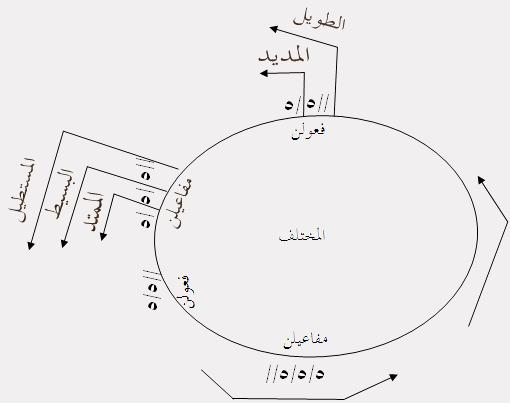
\includegraphics{./Figures/Ch_2_Background/Al-Mokhtalef.jpg}
% \caption{Al-Mokhtalef circle which contains three classes Al-Taweel, Al-Madeed and Al-Baseet}~\label{fig:Circle_Mokhtalef}
%\end{figure}

\item \textbf{Al-Mo'talef \textarabic{المُؤْتَلِف}}: This group contains two classes Al-Kamel and Al-Wafer. Table~\ref{tab:Al-Mo'talef_Group} shows this relation between them.

\begin{table}[!h]
  \centering
  \begin{tabular}{c c c}
    \hline
    \textbf{\#} & \textbf{Meter}  & \textbf{Feet} \\
    \hline
    1 & \textarabic{Al-Wafer} & \textarabic{مُفَاعَلَتُنْ مُفَاعَلَتُنْ مُفَاعَلَتُنْ}\\
    2 &\textarabic{Al-Kamel}&  \textarabic{مُتَفَاعِلُنْ مُتَفَاعِلُنْ مُتَفَاعِلُنْ}\\
    \hline                                                
  \end{tabular}
\caption{Al-Mo'talef Circle Group.}\label{tab:Al-Mo'talef_Group}
\end{table}
  
%\begin{figure}[H]
%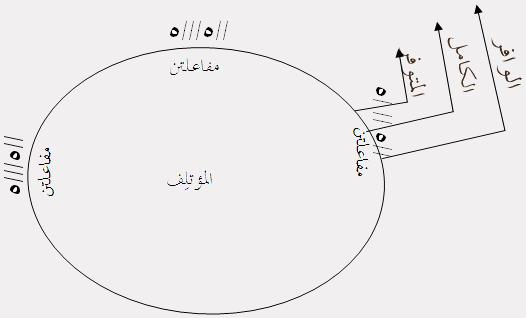
\includegraphics{./Figures/Ch_2_Background/Al-Mo'talef.jpg}
%\caption{Al-Mo'talef circle which contains three classes Al-Kamel and Al-Wafer}~\label{fig:Circle_Motalef}
%\end{figure}


\item \textbf{Al-Mojtaleb \textarabic{المُجْتَلَب}}: This group contains three classes Al-Raml, Al-Rejz and Al-Hazaj. Table~\ref{tab:AlMojtaleb_Group} shows this relation between them.


\begin{table}[!ht]
  \centering
  \begin{tabular}{c c c}
    \hline
    \textbf{\#} & \textbf{Meter Name}  & \textbf{Feet} \\
    \hline
    1 & \textarabic{Al-Raml} & \textarabic{فَاعِلاتُنْ فَاعِلاتُنْ فَاعِلاتُنْ}\\
    2 &\textarabic{Al-Rejz}&  \textarabic{مُسْتَفْعِلُنْ مُسْتَفْعِلُنْ مُسْتَفْعِلُنْ}\\
    3 &\textarabic{Al-Hazaj}  & \textarabic{مَفَاعِيْلُنْ مَفَاعِيْلُنْ مَفَاعِيْلُنْ}\\
    \hline                                                
  \end{tabular}
\caption{Al-Mojtaleb Circle Group.}\label{tab:AlMojtaleb_Group}
\end{table}
    
  
%\begin{figure}[H]
%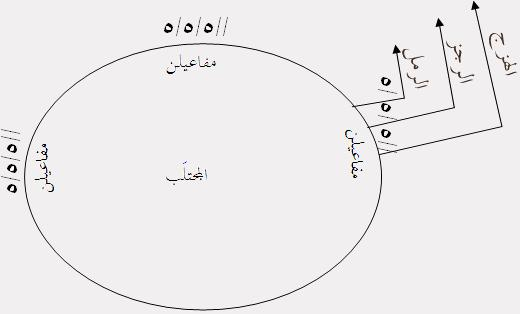
\includegraphics{./Figures/Ch_2_Background/Mojtaleb.jpg}
%\caption{Al-Mojtaleb circle which contains three classes }~\label{fig:Circle_Mojtaleb}
%\end{figure}


\item \textbf{Al-Moshtabeh \textarabic{المُشْتَبِه}}: This group contains six classes Al-Sarea, Al-Monsareh, Al-Khafeef, Al-Modarea, Al-Moktadeb and Al-Mojtaz. Table~\ref{tab:AlMoshtabeh_Group} shows this relation between them.


\begin{table}[!ht]
  \centering
  \begin{tabular}{c c c}
    \hline
    \textbf{\#} & \textbf{Meter Name}  & \textbf{Feet} \\
    \hline
    1 & \textarabic{Al-Sarea} & \textarabic{مُسْتَفْعِلُنْ مُسْتَفْعِلُنْ مَفْعُولاتُ}\\
    2 &\textarabic{Al-Monsareh}&  \textarabic{مُسْتَفْعِلُنْ مَفْعُولاتُ مُسْتَفْعِلُنْ}\\
    3 &\textarabic{Al-Khafeef}  & \textarabic{فَاعِلاتُنْ مُسْتَفْعِلُنْ فَاعِلاتُنْ}\\
    4 &\textarabic{Al-Modarea}  & \textarabic{مَفَاعِيْلُنْ فَاعِلاتُنْ مَفَاعِيْلُنْ}\\
    5 &\textarabic{Al-Moktadeb}  & \textarabic{مَفْعُولاتُ مُسْتَفْعِلُنْ مُسْتَفْعِلُنْ}\\
    6 &\textarabic{Al-Mojtaz}  & \textarabic{مُسْتَفْعِ لُنْ فَاعِلاتُنْ فَاعِلاتُنْ}\\
    \hline                                                
  \end{tabular}
\caption{Al-Moshtabeh Circle Group.}\label{tab:AlMoshtabeh_Group}
\end{table}
    
  
%\begin{figure}[H]
%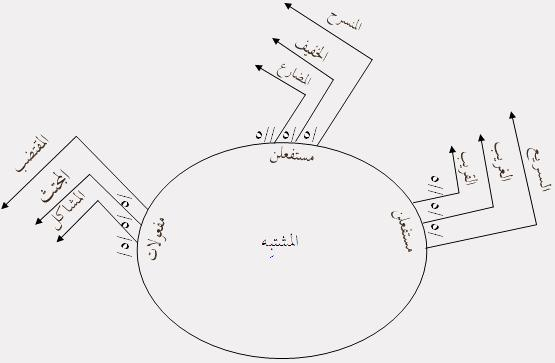
\includegraphics{./Figures/Ch_2_Background/Al-Moshtabeh.jpg}
%\caption{Al-Moshtabeh circle which contains six classes Al-Sarea, Al-Monsareh, Al-Khafeef, Al-Modarea, Al-Moktadeb and Al-Mojtaz }~\label{fig:Circle_AlMoshtabeh}
%\end{figure}


\item \textbf{Al-Motafeq \textarabic{المُتَّفِق}}: This group contains two classes Al-Motaqareb and Al-Motadarek. Table~\ref{tab:AlMotafeq_Group} shows this relation between them.

\begin{table}[!ht]
  \centering
  \begin{tabular}{c c c}
    \hline
    \textbf{\#} & \textbf{Meter}  & \textbf{Feet} \\
    \hline
    1 & \textarabic{Al-Motaqareb} & \textarabic{فَعُولُنْ فَعُولُنْ فَعُولُنْ فَعُولُنْ}\\
    2 &\textarabic{Al-Motadarek}&  \textarabic{فَاعِلُنْ فَاعِلُنْ فَاعِلُنْ فَاعِلُنْ}\\
    \hline                                                
  \end{tabular}
\caption{Al-Motafeq Circle Group.}\label{tab:AlMotafeq_Group}
\end{table}
   
%\begin{figure}[H]
%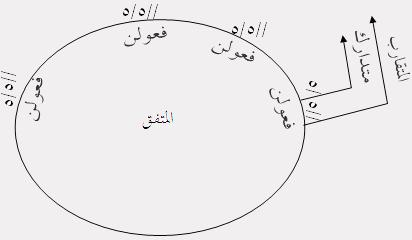
\includegraphics{./Figures/Ch_2_Background/Al-Motafeq.jpg}
%\caption{Al-Motafeq circle which contains six classes Al-Motaqareb and Al-Motadarek}~\label{fig:Circle_Motafeq}
%\end{figure}


\end{itemize}




%%% Local Variables:
%%% mode: latex
%%% TeX-master: "../master"
%%% TeX-engine: xetex
%%% End:
